% begin_generated_IBM_copyright_prolog                             %
%                                                                  %
% This is an automatically generated copyright prolog.             %
% After initializing,  DO NOT MODIFY OR MOVE                       %
% ================================================================ %
%                                                                  %
% (C) Copyright IBM Corp.  2011, 2011                              %
% Eclipse Public License (EPL)                                     %
%                                                                  %
% ================================================================ %
%                                                                  %
% end_generated_IBM_copyright_prolog                               %
\documentclass[conference]{IEEEtran}

% the IEEEpubid command is disabled by default for conference styles for some odd reason
% this command enables it...
\IEEEoverridecommandlockouts

%\IEEEpubid{978-1-4244-9705-8/10/\$26.00 \copyright 2010 IEEE}
\IEEEpubid{\makebox[\columnwidth]{978-1-4244-9705-8/10/\$26.00 ~\copyright~2010 IEEE\hfill}
\hspace{\columnsep}\makebox[\columnwidth]{}}

\usepackage[pdftex]{graphicx}
\usepackage{url}

\begin{document}

\title{Blue Gene/Q Resource Management Architecture}

\author{\IEEEauthorblockA{Tom Budnik, Brant Knudson, Mark Megerian, Sam Miller, Mike Mundy, Will Stockdell}\\
IBM Systems and Technology Group, Rochester, MN\\
Email: \{tbudnik, bknudson, megerian, samjmill, mmundy, stockdel\}@us.ibm.com}

\maketitle

\begin{abstract}
% begin_generated_IBM_copyright_prolog                             %
%                                                                  %
% This is an automatically generated copyright prolog.             %
% After initializing,  DO NOT MODIFY OR MOVE                       %
% ================================================================ %
%                                                                  %
% (C) Copyright IBM Corp.  2011, 2011                              %
% Eclipse Public License (EPL)                                     %
%                                                                  %
% ================================================================ %
%                                                                  %
% end_generated_IBM_copyright_prolog                               %
As supercomputers scale to a million processor cores and beyond, the underlying resource management
architecture needs to provide a flexible mechanism to manage the wide variety of workloads executing on the
machine. In this paper we describe the novel approach of the Blue Gene/Q (BG/Q) supercomputer in addressing
these workload requirements by providing resource management services that support both the high performance
computing (HPC) and high-throughput computing (HTC) paradigms. We explore how the resource management
implementations of the prior generation Blue Gene (BG/L and BG/P) systems evolved and led us down the path to
developing services on BG/Q that focus on scalability, flexibility and efficiency. Also provided is an
overview of the main components comprising the BG/Q resource management architecture and how they interact
with one another. Introduced in this paper are BG/Q concepts for partitioning I/O and compute resources to
provide I/O resiliency while at the same time providing for faster block (partition) boot times. New features, such as
the ability to run a mix of HTC and HPC workloads on the same block are explained, and the advantages of this
type of environment are examined. Similar to how Many-task computing (MTC) \cite{raicu:08} aims to combine elements of HTC
and HPC, the focus of BG/Q has been to unify the two models in a flexible manner where hybrid workloads
having both HTC and HPC characteristics are managed simultaneously.

\end{abstract}

% begin_generated_IBM_copyright_prolog                             %
%                                                                  %
% This is an automatically generated copyright prolog.             %
% After initializing,  DO NOT MODIFY OR MOVE                       %
% ================================================================ %
%                                                                  %
% (C) Copyright IBM Corp.  2011, 2011                              %
% Eclipse Public License (EPL)                                     %
%                                                                  %
% ================================================================ %
%                                                                  %
% end_generated_IBM_copyright_prolog                               %
\section{Introduction}
Blue Gene/Q (BG/Q) is the third generation computer architecture in the Blue Gene family of supercomputers. 
The BG/Q system will be capable of scaling to over a million processor cores while making the trade-off of 
lower power consumption over raw processor speed.

Blue Gene systems are connected to multiple communications networks. BG/L, the first generation member of the
Blue Gene supercomputers, and BG/P, the second generation, both provide a three dimensional (3D) torus network that is used for peer-to-peer
communication between compute nodes. BG/Q advances the technology by supporting a five dimensional (5D) torus network. All the Blue Gene 
systems incorporate a collective network for collective communication operations and a global interrupt network for fast barriers.
An Ethernet network provides communication to external I/O attached to Blue Gene while a private Ethernet network
provides access for managing hardware resources.   

By default a custom lightweight operating system called Compute Node Kernel (CNK) is loaded on compute nodes while I/O nodes
run the Linux operating system. I/O nodes were integrated on the same board as compute nodes for BG/L and BG/P. The BG/Q
hardware design moves the I/O nodes to separate I/O drawers and I/O racks.

Just as the Blue Gene hardware has advanced over multiple generations, the resource management software on Blue Gene 
known as the Control System has also evolved to support the latest supercomputer workload models.

This position paper describes the BG/Q resource management software design at an early stage of development.
While the software architecture is in place, the development team is not able to share performance results
with the community at this point in time.

% begin_generated_IBM_copyright_prolog                             %
%                                                                  %
% This is an automatically generated copyright prolog.             %
% After initializing,  DO NOT MODIFY OR MOVE                       %
% ================================================================ %
%                                                                  %
% (C) Copyright IBM Corp.  2011, 2011                              %
% Eclipse Public License (EPL)                                     %
%                                                                  %
% ================================================================ %
%                                                                  %
% end_generated_IBM_copyright_prolog                               %
\section{History of Blue Gene Workloads}

\subsection{First Generation Blue Gene (BG/L aka Blue Gene ``Light'')}
\label{sec:BGL}

Highlights/Features:
\begin{itemize}
\item Initial release supports HPC Message Passing Interface (MPI) workloads and jobs occupy multiples of 512 compute nodes.
\item Second release supports running HPC jobs on as few as 32 compute nodes.
\item Third release adds limited support for HTC single-node jobs.
\end{itemize}

The term ``light'' indicated that this was the first, smallest, and therefore ``light'' version of a
new supercomputer architecture that would grow into larger and more powerful designs in the future.
The stated goal of BG/L was to enable massively parallel applications to run at unprecedented
scales. The flagship BG/L machine, developed in a partnership between IBM and Lawrence Livermore
National Laboratory (LLNL), consisted of 64 racks of compute hardware, comprising 65,536 compute
nodes, and 131,072 processor cores. This machine achieved the top spot on the Top500 list of
supercomputers in November of 2004 \cite{website:top500November2004}, and held that position for an
unprecedented seven consecutive lists after being expanded to 104 racks. The machine was built for
scaling large applications, with relatively little emphasis placed on running many small jobs. In
Blue Gene, the term ``block'' is used to describe how the machine hardware is partitioned into
groups of compute nodes or I/O nodes. Collections of I/O nodes on BG/Q are referred to as ``I/O
blocks'' and collections of compute nodes are referred to as ``compute blocks''. In BG/L and BG/P
systems, only compute blocks existed and were simply called blocks. In
the initial design of the machine, the smallest block of the machine that could be used to run a job
was 512 compute nodes, or a half rack. Furthermore, a job had to occupy the entire block. This was
not considered to be a significant limitation, since the machine was designed with a priority of
running large jobs, and with a 64 rack machine one could run as many as 128 simultaneous jobs.
However, many customers expressed an interest in smaller machines, and some required only a single
rack system. It became clear that the smaller machines would require the ability to subdivide the
system in units with less than 512 compute nodes.  Software features were added to enable blocks
containing as few as 32 compute nodes. This was a significant enhancement to the usability of the
machine. The Blue Gene architecture suddenly became relevant to customers that would conceivably
never run a job that occupied the entire machine, and had workloads that did not scale to thousands
of parallel tasks. Now they could subdivide the machine into many smaller blocks, and run many
simultaneous jobs, and still get the benefits of a Blue Gene, such as the compute density of 1,024
compute nodes in a single rack, and the unparalleled power efficiency.

Even with the features added to enable smaller blocks, each job still had to be a parallel,
multi-node job. MPI based programs had to be equipped to break a problem down into multiple, smaller
pieces of work. This was always the stated purpose of the Blue Gene architecture, and yet there was
customer interest in expanding its use to other workloads, and not all of those workloads used MPI.

Also, there was still a requirement that each block had to contain at least one I/O node connected
to the functional network to enable I/O. This was a hardware limitation due to the collective network
used by the compute nodes to communicate with the I/O node. This meant that in order to create the smallest blocks of
32 compute nodes, a rack of 1,024 compute nodes had to be equipped with 32 I/O nodes. This was not a
common machine configuration for BG/L, since most customers chose a ratio of only 8 or 16 I/O nodes
per rack, due to hardware costs and Ethernet switch capacity. As a result, even though 32 node
blocks were enabled by the software, there were not many installed racks of BG/L that had the
hardware configured to take advantage of this feature.

So there remained a need to enable more simultaneous jobs on BG/L, and to somehow circumvent the
hardware limitations that required an I/O node per job. With these goals in mind, further work was
done on BG/L to enable rudimentary support for HTC style applications  \cite{marshall:09}. The
strength of BG/L was in its robust performance of parallel applications, and it was best known as an
extreme scaling HPC machine. However, some customers started to consider the possibility of using
BG/L as a cluster of many small nodes, each running independent tasks. This was very different than
anything that had been done on a BG/L machine, and not something that the Control System software
was equipped to handle. As a proof-of-concept, a group of software engineers created an HTC model
that could be achieved by executing a \emph{launcher} program on all of the compute nodes of a BG/L
block. From the perspective of the Control System, this was a single binary executable started on
all of the compute nodes in a block, so at that level, it was no different than a typical HPC
application. But this \emph{launcher} program was really just a basic mechanism to execute different
applications on different compute nodes using special support in the CNK \cite{peters:08}. While
this model demonstrated a method of running many different executables on a single BG/L block, it
had several key limitations that made its widespread adoption impractical. One drawback was that the
Control System was unaware of the different applications running and had no way to do tracking and
accounting of the individual jobs. Because of the \emph{launcher} based design, jobs could not be
signaled or killed and it was impossible to separate any job output written to standard output.
Also, all of the launched jobs were run under the same user which was a security limitation.

This initial proof-of-concept showed that it was possible for Blue Gene to handle both ends of the spectrum. The worlds largest parallel jobs as well as the smallest single-node jobs could be supported by the Blue Gene architecture. It also became apparent that tighter integration with the Control System and kernel layer would be necessary for HTC workloads to be widely accepted on Blue Gene.

\subsection{Second Generation Blue Gene (BG/P aka Blue Gene ``Petaflop'')}
\label{sec:BGP}

Highlights/Features:
\begin{itemize}
\item Stronger integration for HTC workloads in Control System and kernel layer.
\item Lightweight HTC job submission design along with a multiplexer to handle thousands of job proxy client connections.
\end{itemize}

BG/P was designed as a petaflop capable machine and the flagship 72 rack system has a theoretical peak
performance of one petaflop \cite{website:jugene}. There were many new features and enhancements made in BG/P.
One of the key new software elements was an HTC job submission mode that was fully integrated into the Control
System software. Figure \ref{fig:htcjobsubmission} shows the architecture and various components. This meant
that unlike the BG/L \emph{launcher} design, the BG/P design could allow users to submit single task jobs to
nodes within a block. Because the Control System was fully aware of every HTC job being run, each job could be
tracked and accounted for in the job history, output from jobs were not intermingled, and each job had a
distinct user associated with it. Several novel software ideas emerged from this HTC project due to the need
for fast and efficient job launch time. When running thousands of HTC style jobs, this setup time was a
critical factor and often dominated the total perceived execution time of the job itself. Due to this, much
focus was placed on providing a fast, lightweight, and efficient job submission path. The addition of a
multiplexer component on the job submission nodes, as well as I/O nodes, reduced the authentication overhead
and offloaded several verification tasks from the central daemon. Using prepared SQL statements to insert,
update, and remove entries from the database proved much more efficient than using dynamic queries.

\begin{figure}[!b]
    \centering
    \caption{BG/P HTC Job submission architecture.}
    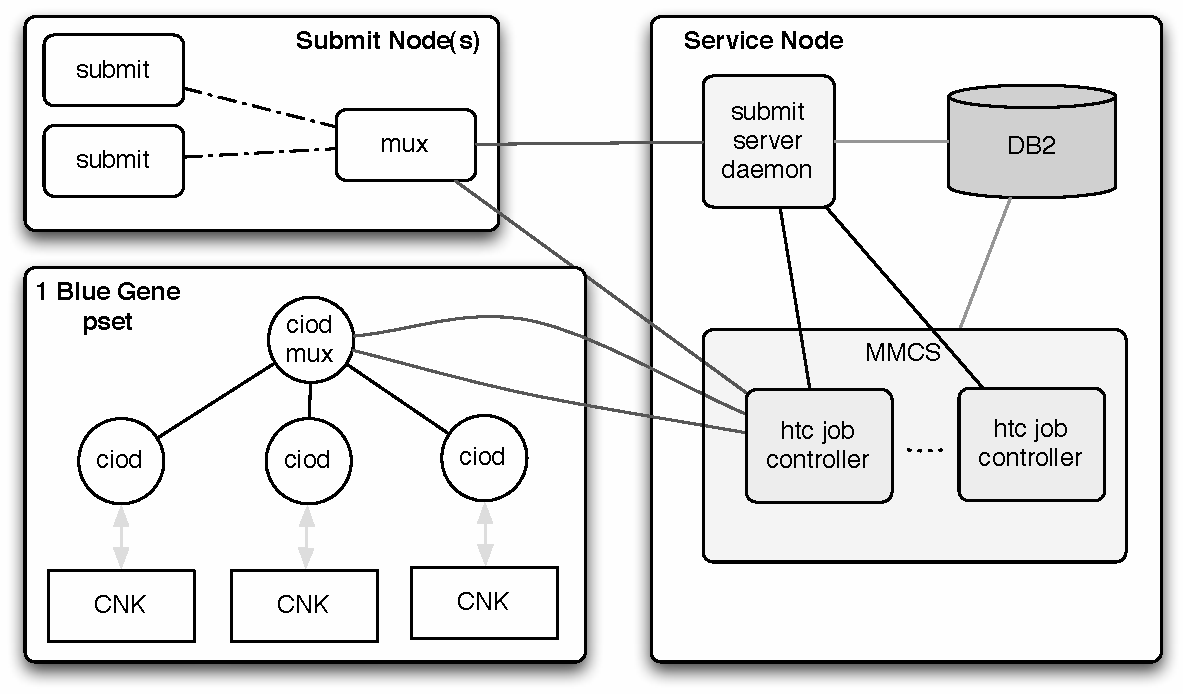
\includegraphics[width=3.5in]{bgp_htc_architecture}
    \label{fig:htcjobsubmission}
\end{figure}

Rather than being a proof-of-concept project like the BG/L version of HTC, the BG/P HTC software was
production level. This made a BG/P machine much more flexible in terms of the workloads that it could support.
A machine could be used for part of the day running massively parallel HPC applications, then spend another
part of the day processing thousands of independent tasks for an HTC workload. Even a blend of HTC and HPC
applications could be running simultaneously on different blocks of the system.

The HTC features of BG/P have been used by many customers, and have indeed expanded the scope of possible
workloads that can run on Blue Gene. However, the work in this HTC space still left room for improvement. The
BG/P system software was restricted in an artificial way because a block could handle either single node HTC jobs or
HPC (MPI) type jobs but not a blend of the two. In order to switch between workload styles a block required
rebooting which was inefficient. For complete flexibility the ideal solution would be for a block to handle
all types of workloads without a reboot. Another area of concern was the multiple conflicting methods of job
submission. For HPC style jobs the \emph{mpirun} command was invoked, for HTC type jobs the \emph{submit}
command was used. The grand unification of multiple commands into a single comprehensive job submission
command would have to wait though until BG/Q when the Control System software could be restructured. 

% begin_generated_IBM_copyright_prolog                             %
%                                                                  %
% This is an automatically generated copyright prolog.             %
% After initializing,  DO NOT MODIFY OR MOVE                       %
% ================================================================ %
%                                                                  %
% (C) Copyright IBM Corp.  2011, 2011                              %
% Eclipse Public License (EPL)                                     %
%                                                                  %
% ================================================================ %
%                                                                  %
% end_generated_IBM_copyright_prolog                               %
\section {Third Generation Blue Gene (BG/Q)}

Highlights/Features:
\begin{itemize}
\item Resilient I/O framework providing higher availability for workloads.

\item Flexible workload architecture allowing not just single task (HTC) or entire block (HPC), but the 
full range of intermediate sizes including the ability to run multiple HPC (MPI) jobs on a single block.

\item Unification of multiple job submission models into an all-encompassing job submission command based 
on a client-multiplexer-server infrastructure.

\item Breaking the reliance of having an I/O node per block which is motivated by a higher ratio of compute 
nodes per I/O node. 

\end{itemize}

The latest supercomputer in the Blue Gene series is BG/Q which aims to reach multiple petaflops scaling 
when it is delivered. The archetypal BG/Q system called Sequoia will be installed at LLNL as a part of the 
Advanced Simulation and Computing Program. It will consist of 98,304 compute nodes comprising 1.6 million 
processor cores in 96 racks \cite{website:sequoia}.

\subsection{I/O resiliency}
\label{sec:io}
A significant change in the I/O architecture occurs with BG/Q and it brings significantly higher levels of 
resiliency and availability to Blue Gene workloads. Prior Blue Gene systems provided I/O nodes integrated on
the same board as compute nodes. For BG/Q the I/O nodes are now located on separate I/O drawers and I/O racks. 
With this hardware change, that at first appears to make the machine hardware less flexible, comes the 
opportunity to refactor the system software in a manner that actually makes it more flexible and resilient 
than the predecessor machines. This objective is achieved by BG/Q permitting hardware I/O resources to be 
booted independently of hardware compute resources. Previous Blue Gene generations would boot both the I/O
and compute resources present in a block and I/O issues could cause the entire block to fail causing any 
active jobs to be terminated. With BG/Q having the ability to mount file systems in a persistent manner, 
and not remounted every time a compute block is booted, comes the benefits of faster boot times and less 
start-up traffic to the file systems. In addition, new software functionality exists to allow for some 
degree of failing I/O nodes in an I/O block. When an I/O malfunction occurs the software will attempt to
re-route I/O traffic to other working I/O nodes and make efforts to recover the failed I/O nodes automatically. 
When successful the recovered nodes are placed back into service without any administrative involvement
and total transparency to running applications.  The only impact would be some degradation in overall
I/O performance for the application. This is very important when enabling many-task computing on 
Blue Gene. The added feature of I/O node 
failure resiliency means that all compute nodes remain active and eligible to run jobs, even in the 
face of a failure on an I/O node.  In the previous design on BG/P, the failure of an I/O node would 
render all connected compute nodes ineligible to run tasks.

\begin{figure}[!t]
    \centering
    \caption{BG/Q Job submission architecture.}
    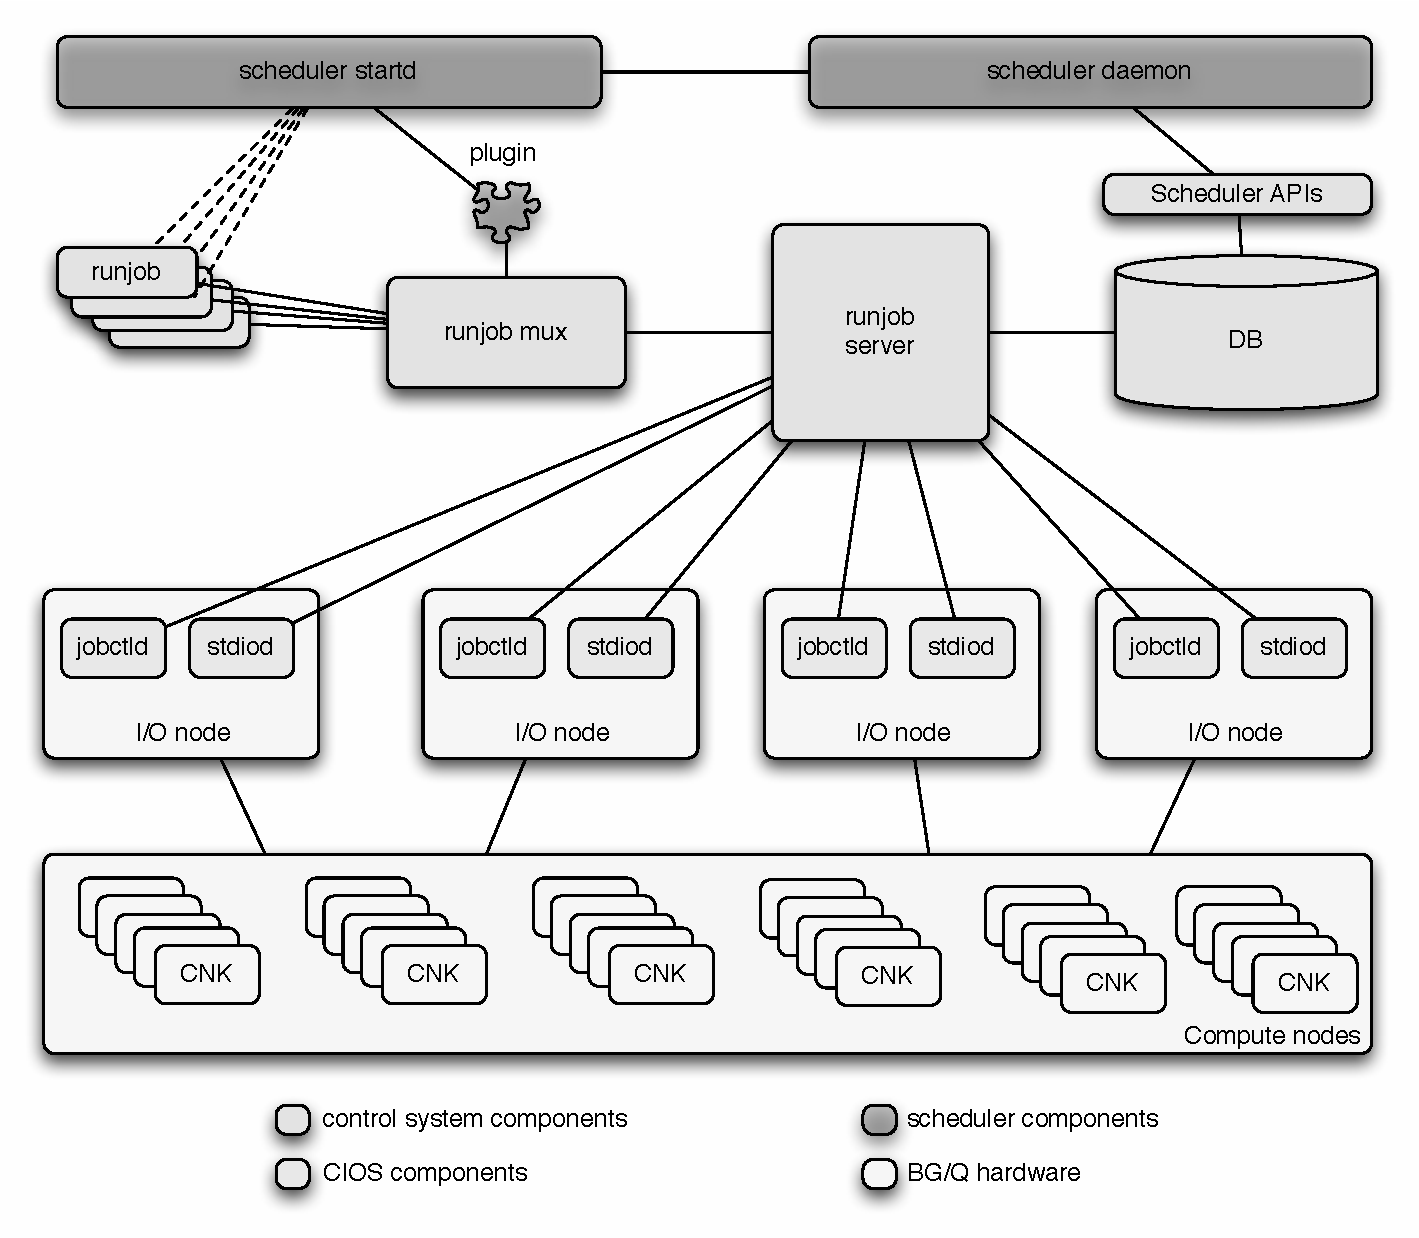
\includegraphics[width=3.5in]{jobsubmission}
    \label{fig:bgqjobsubmission}
\end{figure}

\subsection{Job Submission}
\label{sec:bgqjobsubmission}

The job submission architecture, shown in Figure \ref{fig:bgqjobsubmission}, has changed significantly 
when compared to the previous generation systems. It is somewhat based on the HTC job submission architecture 
shown in Figure \ref{fig:htcjobsubmission}. The most notable difference is the unification of HTC and HPC 
job submission components from BG/L and BG/P systems into a single consistent interface. The architecture 
also more closely resembles the HTC job submission architecture described in section \ref{sec:BGP} rather 
than the \emph{mpirun} or \emph{launcher} architecture described in section \ref{sec:BGL}.

Although the architecture is different, the objective and design goals of these job launch components are 
largely the same as previous designs. 

\begin{itemize}
\item{Fast and scalable job launch}
\item{Transparently relay standard output}
\item{Maintain state in a database}
\end{itemize}

\noindent
Three primary job submission components shown in Figure \ref{fig:bgqjobsubmission} help achieve these 
objectives. The \emph{runjob} component acts as a shadow of the job, its purpose is to parse arguments from 
the user or scheduler describing the job's resource requirements. Conceptually it performs the same actions 
as \emph{mpirun} or \emph{submit} from previous generation Blue Gene systems. Typically this component is 
executed under the user's credentials. The \emph{runjob\_mux} component acts as a traffic cop and gatekeeper. 
It obtains credentials from the \emph{runjob} component and performs some validation and sanity checking 
before forwarding the request to the \emph{runjob\_server}. The \emph{runjob\_server} component performs 
arbitration on the nodes each job has requested to use. This capability is significantly different than 
arbitration done by \emph{mpirun} due to the additional requirements imposed by sub-block jobs, which are 
described in section \ref{sec:subblockjobs}. The \emph{runjob\_server} also maintains job state in a database. 
Both the \emph{runjob\_mux} and \emph{runjob\_server} are executed under administrative credentials like 
the rest of the Control System.

\subsection{Compute Node Kernel}
\label{sec:cnk}
For BG/Q, job management in the CNK is more flexible compared to BG/P. As described in section \ref{sec:BGP}, 
a BG/P block is booted in a specific mode and CNK allocates and configures resources once.  There is no way to 
reconfigure resources without rebooting the block.  For BG/Q, the CNK allocates and configures resources with 
each job.  When a job is started, CNK is given information about the size and shape of the compute nodes 
participating in the job.  CNK uses that information to configure resources dynamically with each job.  
For example, a class route for the collective network that includes all of the nodes in the job is 
calculated with each job. This is equivalent to a MPI COMM\_WORLD communicator.  With I/O nodes located
on separate I/O blocks and CNK uses a service model for I/O instead of being hard-wired to a specific I/O node on 
the board.  This allows CNK to dynamically change which I/O node it uses for I/O services.

\subsection{Sub-block Jobs}
\label{sec:subblockjobs}

\begin{figure}[!b]
    \centering
    \caption{BG/Q Sub-block jobs.}
    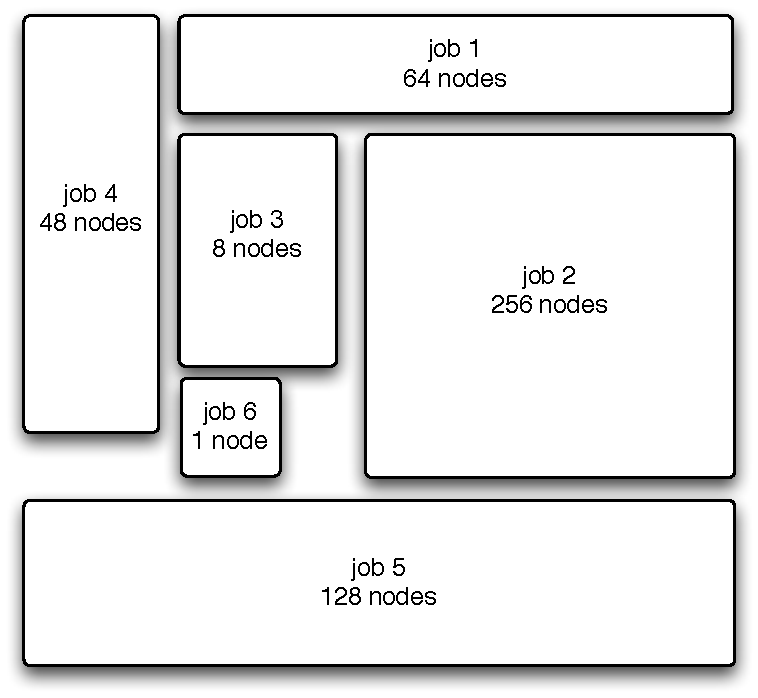
\includegraphics[width=3.5in]{subblockjobs}
    \label{fig:subblockjobs}
\end{figure}

While the concept of running multiple jobs on a single compute block was available on a BG/P system by
booting the block in HTC mode, it was limited to single node jobs without any ability to utilize the collective
networks between compute nodes. This concept is certainly useful for certain workloads, but the lack of a 
dedicated high speed communication network is severely limiting for many others. On previous Blue Gene systems,
messaging communication between multiple compute nodes within a job was only possible by using all of the compute nodes
in the entire block and idling the unused compute nodes should a job not need all them. This often led to 
significant fragmentation and under-utilization of the system when presented with a workload of thousands of 
jobs each needing a handful of compute nodes.

To address this problem, we describe a new software feature in BG/Q that we have termed \emph{sub-block jobs}.
This capability is enabled by the dynamic job configuration performed by CNK described in section \ref{sec:cnk},
and the physical separation of I/O and compute hardware described in section \ref{sec:io}. A sub-block job differs
from a job using the entire block by requesting a compute node corner location and five
dimensional shape at job launch time. This corner and shape are combined to logically create a sub-block, which
is then used for resource arbitration to ensure overlapping compute nodes are not in use by active jobs. It is 
also used to enforce the job is entirely contained within the corner compute node's midplane. Using a shape 
effectively enforces a collection of compute nodes without any holes, easing the challenges this would otherwise pose for the messaging 
communications software stack. The shape of a sub-block job has a maximum size of 512 compute nodes. This limitation is 
solely imposed by software and not due to a hardware limitation. The logic beind this restriction is a 512 node midplane is the 
building block for creating larger blocks. Doing so also greatly simplifies the resource arbitration. Any shape,
between a single node (1x1x1x1x1) and the entire midplane (4x4x4x4x2), is a valid shape for a sub-block job. Most
importantly, job sizes are not limited to a power of two, or by any artificial I/O ratio. 

Figure \ref{fig:subblockjobs} shows a two dimensional layout of six sub-block jobs using a variety of corner
and shape combinations. It is important to note the compute nodes in the empty space between the logical layout of the
jobs are available for use. They are not orphaned, reserved, or idled by another job.

There are several application considerations when using sub-block jobs. Foremost, the I/O resources are shared with other jobs 
serviced by the same I/O node. Considering the six jobs shown in Figure \ref{fig:subblockjobs}, one job could 
monopolize resources on the I/O node. If any of the five remaining jobs need guaranteed I/O bandwidth, 
precautions may need to be taken by the scheduler to ensure adequate resources are available. Secondly, sub-block jobs 
do not have the same electrical isolation guarantee that their full-block job counterparts do. On all Blue Gene systems, 
a block of compute nodes is electrically isolated from neighboring compute nodes when it is booted. Since sub-block jobs are 
sharing the same compute node to I/O node bridge, this guarantee cannot be enforced. This can be a security
concern to certain applications if they have a requirement to not share the torus links between compute nodes.

\subsection{Scalability}
\label{sec:scalability}
As described in section \ref{sec:bgqjobsubmission}, the job submission framework shown in Figure \ref{fig:bgqjobsubmission} 
is an enhanced extension of the HTC job submission architecture from BG/P shown in Figure \ref{fig:htcjobsubmission}. 
This is
\vfill\break
%spacing inplace to equalize column lengths on last page
%this must be done by hand

\noindent
in part due to the scaling strengths proven with that architecture. We anticipate 
this scalable design will be capable of handling workloads of tens of thousands of simultaneous jobs.

% begin_generated_IBM_copyright_prolog                             %
%                                                                  %
% This is an automatically generated copyright prolog.             %
% After initializing,  DO NOT MODIFY OR MOVE                       %
% ================================================================ %
%                                                                  %
% (C) Copyright IBM Corp.  2011, 2011                              %
% Eclipse Public License (EPL)                                     %
%                                                                  %
% ================================================================ %
%                                                                  %
% end_generated_IBM_copyright_prolog                               %
\section{Conclusion}

Many-Task Computing describes an emerging application style for large scale computing. 
It cuts across both HTC and HPC application paradigms but has sufficient enough 
characteristics to warrant its own classification as a computing paradigm. In this
paper we have described how Blue Gene architecture has transitioned from the original
BG/L machine that
specialized in large scale HPC workloads to the latest BG/Q system that will be able to tackle 
a multitude of 
customer's MTC workloads under a unified 
Control System software model. BG/Q is just a way station on the journey to exaflop 
supercomputing though. New challenges and workloads await and the Blue Gene architecture 
must continue to evolve to meet the future requirements of exaflop computing. 
With a sustained record of success in supercomputing, all indications point 
to the fact that the elegant and flexible architecture of Blue Gene is prepared 
to meet those challenges. 



\bibliographystyle{IEEEtran}
\bibliography{bibliography}

% that's all folks
\end{document}

